

\chapter{جمع بندی}

حوزه خودروهای خودران پیشرفت چشمگیری داشته است، اما هنوز هم دامنه پیشرفت زیادی در آینده دارد. 
\cite{paliwal2023survey}
در ابتدا تکنیک‌های مختلف برنامه‌ریزی حرکتی را ارائه کرد که تمرکز اصلی آن بر روی الگوریتم جستجوی
 \lr{A* }
  و تغییرات آن بود. چندین گونه از الگوریتم  \lr{A* } مورد بررسی قرار گرفت و نشان داده شد که چگونه این تغییرات به حل مسائل با الگوریتم کلاسیک \lr{ A *} کمک می کند. بسیاری از تغییرات الگوریتم  \lr{A* } را می توان در آینده با بهینه سازی الگوریتم کلاسیک یا انواع آن توسعه داد و آزمایش کرد. یکی از این تغییرات بالقوه، اصلاح تابع اکتشافی مورد استفاده در این الگوریتم‌ها است. نویسنده امیدوار است که این مقاله در ارائه یک نمای کلی از انواع مختلف الگوریتم  \lr{A* } موفق باشد، که می تواند به عنوان مرجع در حین کار بر روی انواع جدید برای ارائه عملکرد بهتر نسبت به الگوریتم های برنامه ریزی حرکتی موجود استفاده شود.
در روش های متفاوت که بررسی شد ورژن هندسی الگورییتم 
\lr{A*}
برای زمانی مطلوب است که نیاز به مسیری تاحد امکان صاف داریم و در این حالت الگوریتم هندسی با کاهش تعداد گره های گسترده شده زمان یافتن مسیر بهینه را به شدت کاهش می دهد . از مزایای آن می توان این موارد را نام برد:
تعداد کمتری از گره ها را گسترش می دهد ،
محاسبه مسیرهای کوتاهتر از \lr{A* }کلاسیک ،
مسیرهای هموارتر و واقعی تر را ایجاد می کند، 
و برای وسایل نقلیه خودران مناسب است .
الگوریتم 
\lr{improved A*}
مسیر کوتاه تری را نسبت به حالت کلاسیک در مسئله ی بررسی شده در مقاله پیدا کرد اما زمانی بیشتر صرف شد . بنابراین زمان اجرا می توند نقطه ضعف این الگوریتم باشد .
الگوریتم های دیگر مثل 
\lr{ARA*} 
و
\lr{ADA*}
زمان اجرا را بسیار پایین می آورددند و بسیار برای کاربرد های برخط مناسب اند .
همین طور 
\lr{Anytime Dynamic A* (AD*)} 
و
\lr{ADA*}
برای محیط های پویا مناسب اند .در 
\ref{conclusion}
 می توانید یک نمای کلی از نظر تعدا گره های گسترش یافته برای هریک از الگوریتم ها در یک مسئله خاص مشاهده نمایید .
 الگوریتم 
 \lr{A*}
 پتانسیل بالایی دارد تا با سایر الگوریتم ها ترکیب شود و الگوریتم هایی با عملکرد زمانی و بهینگی بهتری پدید آورد . به عتوان مثال می توان تابع هیوریستک را تغییر داد یا برای انتخاب هر گره معیار های دیگری نیز افزود ویا ضریب 
 $\epsilon$
 را در طول مسیر تغییر داد و با نزدیک شدن به هدف به سمت 1 برد. 
\begin{figure}[h]
	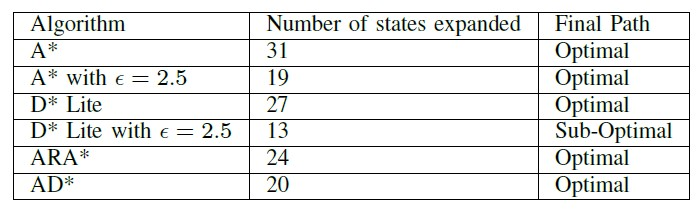
\includegraphics[scale=0.7]{conclusion}
	\centering
	\caption{مقایسه ی گسترش یافته های الگوریتم \lr{A*}}
	\cite{paliwal2023survey}
	\label{conclusion}
\end{figure}
\